\documentclass{article}
\usepackage[top=1in, bottom=1in, left=1in, right=1in]{geometry}
\usepackage{graphicx}
\usepackage{amsmath}
\begin{document}

\begin{flushright}
Matt Jibson \\
EG 520 \\
HW 5
\end{flushright}

\begin{itemize}
	\item[15.1] Problem:
		\begin{displaymath}
			\begin{array}{rl}
				\textrm{maximize} & 2x_1 + x_2 \\
				\textrm{subject to} & 0 \le x_1 \le 2 \\
				& x_1 + x_2 \le 3 \\
				& x_1 + 2x_2 \le 5 \\
				& x_2 \ge 0
			\end{array}
		\end{displaymath}
		Conversion to a minimization done by negation. Add three slack variables. Separate out the first bound into two parts. Hence we have the standard form:
		\begin{displaymath}
			\begin{array}{rl}
				\textrm{minimize} & -2x_1 - x_2 \\
				\textrm{subject to} & x_1 + y_1 = 2 \\
				& x_1 + x_2 + y_2 = 3 \\
				& x_1 + 2x_2 + y_3 = 5 \\
				& x_1 \ge 0, x_2 \ge 0, y_1 \ge 0, y_2 \ge 0, y_3 \ge 0
			\end{array}
		\end{displaymath}
	\item[15.5]
		\begin{displaymath}
			\begin{array}{rl}
				\textrm{minimize} & 2x_1 + 4x_2 + x_3 + 2x_4 \\
				\textrm{subject to} & x_1 + x_2 + x_3 + x_4 = 1000 \\
				& .03x_1 + .08x_2 + .16x_3 + .04x_4 = 100 \\
				& .06x_1 + .46x_2 + .09x_3 + .09x_4 = 20 \\
				& .20x_1 + .05x_2 + .04x_3 = 50 \\
				& x_1 \ge 0, x_2 \ge 0, x_3 \ge 0, x_4 \ge 0
			\end{array}
		\end{displaymath}
		Regarding the existence of a solution to this problem, there is no guarantee that one exists. It is possible that the three percentage requirements have no intersection and thus, since the problem stipulates exact measurements, there is no feasible solution.
	\item[15.8]
		\begin{displaymath}
			\begin{array}{rl}
				\textrm{maximize} & 2x_1 + 5x_2 \\
				\textrm{subject to} & 0 \le x_1 \le 4 \\
				& 0 \le x_2 \le 6 \\
				& x_1 + x_2 \le 8
			\end{array}
		\end{displaymath}
		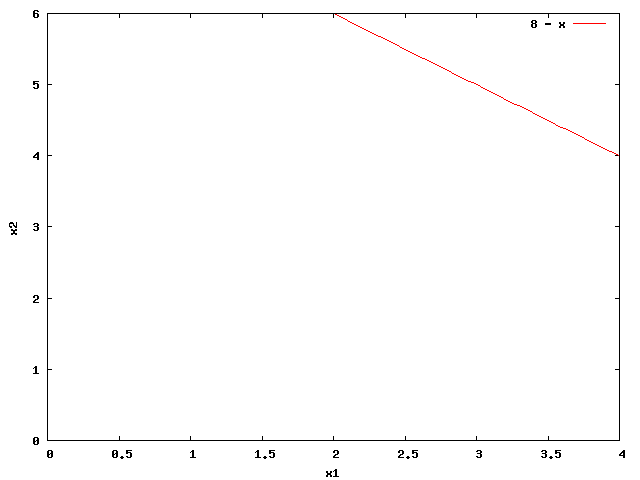
\includegraphics[width=0.5\linewidth]{15-8} \\
		Feasible solutions are edges of the graph, the red line, and not the upper and right edges of the triangle in the upper right corner. From inspection it is clear that the point $(x_1, x_2) = (2, 6)$ is the solution, with a value of $2*2 + 5*6 = 34$.
	\item[16.2] In standard form:
		\begin{displaymath}
			\begin{array}{rl}
				\textrm{minimize} & -x_1 - x_2 - 3x_3 \\
				\textrm{subject to} & x_1 + x_3 = 1 \\
				& x_2 + x_3 = 2 \\
				& x_1, x_2, x_3 \ge 0
			\end{array}
		\end{displaymath}
		The tableau is:
		\begin{displaymath}
			\begin{array}{ccccc}
				& a_1 & a_2 & a_3  & b \\
				& 1 & 0 & 1 & 1 \\
				& 0 & 1 & 1 & 2 \\
				c^T & -1 & -1 & -3 & 0
			\end{array}
		\end{displaymath}
		Which is already in canonical form with respect to the basis $[a_1, a_2]$. Because $r_3$ is the most negative reduced cost coefficient, bring $a_3$ into the basis. Using the ratio test we pivot about the $(1, 3)$th element of the tableau to obtain:
		\begin{displaymath}
			\begin{array}{ccccc}
				& a_1 & a_2 & a_3  & b \\
				& 1 & 0 & 1 & 1 \\
				& 0 & 1 & 1 & 2 \\
				c^T & -1 & -1 & -3 & 0
			\end{array}
		\end{displaymath}
		
		%So:
		%\begin{displaymath}
		%	\begin{array}{cccc}
		%		\mathrm{Variable} & \multicolumn{2}{c}{B^{-1}} & y_0 \\
		%		\hline	
		%	\end{array}
		%\end{displaymath}
	\item[16.3] In standard form:
		\begin{displaymath}
			\begin{array}{rl}
				\textrm{minimize} & -2x_1 - x_2 \\
				\textrm{subject to} & x_1 + x_3 = 5 \\
				& x_2 + x_4 = 7 \\
				& x_1 + x_2 + x_5 = 9 \\
				& x_1, x_2, x_3, x_4, x_5 \ge 0
			\end{array}
		\end{displaymath}
		Start with tableau:
		\begin{displaymath}
			\begin{array}{ccccccc}
				& a_1 & a_2 & a_3 & a_4 & a_5 & b \\
				& 1 & 0 & 1 & 0 & 0 & 5 \\
				& 0 & 1 & 0 & 1 & 0 & 7 \\
				& 1 & 1 & 0 & 0 & 1 & 9 \\
				c^T & -2 & -1 & 0 & 0 & 0 & 0
			\end{array}
		\end{displaymath}
		So begin with BFS $(a_3, a_4, a_5)$.
	\item[16.10]
		\begin{itemize}
			\item [a.]
				For the basis $B = [a_1]$, the basic solution is $x = [1, 0]^T$. \\
				For the basis $B = [a_2]$, the basic solution is $x = [0, 2]^T$.
		\end{itemize}
\end{itemize}

\end{document}